\subsection{3.1 Definition Determinante}{
\vskip1pt

Die Determinante ist eine Zahl, die einer quadratischen Matrix zugeordnet wird und aus ihren Einträgen berechnet werden kann. Die folgenden Spalten/zeileneigenschaften sind Teil ihrer Definition.

\vskip3pt

\textbf{Zeileneigenschaften:}
\vskip2pt

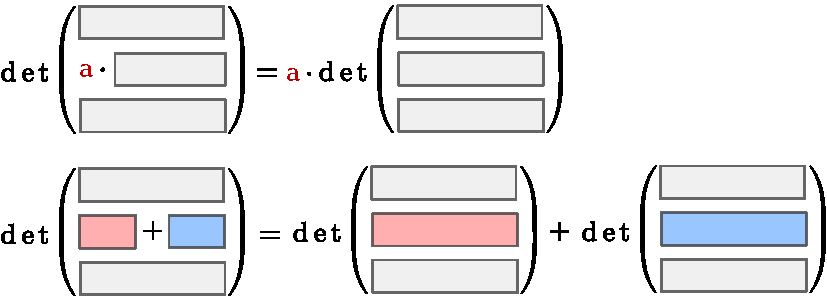
\includegraphics[width = 0.95 \columnwidth]{3_Determinante/Det_Zeilen.pdf}

\begin{itemize}[leftmargin=0.29cm, itemsep=0.5pt]
\item Vertauscht man zwei Zeilen von A, so ändert sich das Vorzeichen der Determinante. 
\item Addiert man ein Vielfaches einer Zeile zu einer anderen, so ändert sich die Determinante nicht.
\end{itemize}

\vskip2pt

\textbf{Spalteneigenschaften:}
\vskip2pt

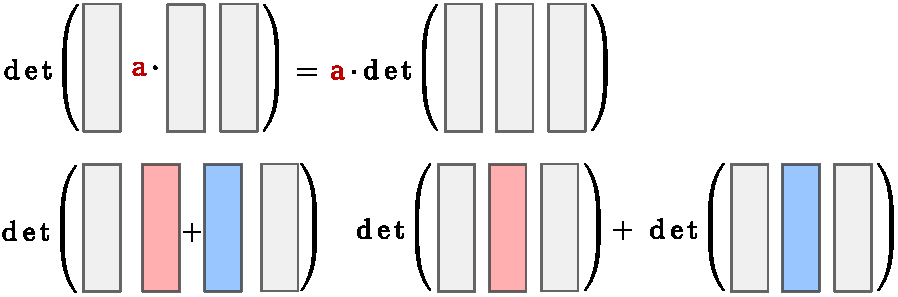
\includegraphics[width = 0.95 \columnwidth]{3_Determinante/Det_Spalten.pdf}

\begin{itemize}[leftmargin=0.29cm, itemsep=0.5pt]
\item Vertauscht man zwei Spalten von A, so ändert sich das Vorzeichen der Determinante. 
\item Addiert man ein Vielfaches einer Spalte zu einer anderen, so ändert sich die Determinante nicht.
\end{itemize}


\vskip2pt

\textbf{Folgerungen aus Zeilen/Spalteneigenschaften:}
\vskip2pt
\begin{itemize}[leftmargin=0.29cm, itemsep=0.5pt]
\item Hat A zwei gleiche Zeilen/Spalten, so gilt $det(A) = 0$.
\item Hat A eine Nullzeile/spalte, so gilt $det(A) = 0$
\item $det(\alpha \cdot A^{n \times n}) = \alpha^n \cdot det(A)$
\end{itemize}

}
\WhiteSpace